% ----------------------
% THIS IS MY DEC1 REPORT
% ----------------------

\documentclass[titlepage,11pt,letterpaper]{article}

\usepackage{graphicx,epsfig,color}
\usepackage{subfigure}
\usepackage{setspace}
\usepackage{amsmath,amssymb}
\usepackage[hang,small,bf]{caption}
\setlength{\captionmargin}{10pt}

\newcommand{\pd}[2]{\frac{\partial#1}{\partial#2}}
% Page Margins
\voffset=-1.0in
\topmargin=0.75in
\headheight=0.0in
\headsep=0.0in
\hoffset=-1.0in
\oddsidemargin=0.7in
\evensidemargin=0.7in

\parindent      0.2000in

\textwidth=7.0in
\textheight=9.25in

% Line Spacing
\renewcommand{\baselinestretch}{1.33}

% Alter some LaTeX defaults for better treatment of figures:
% See p.105 of "TeX Unbound" for suggested values.
    % See pp. 199-200 of Lamport's "LaTeX" book for details.
    %   General parameters, for ALL pages:
    \renewcommand{\topfraction}{0.9}	% max fraction of floats at top
    \renewcommand{\bottomfraction}{0.8}	% max fraction of floats at bottom
    %   Parameters for TEXT pages (not float pages):
   \setcounter{topnumber}{2}
    \setcounter{bottomnumber}{2}
    \setcounter{totalnumber}{4}     % 2 may work better
    \setcounter{dbltopnumber}{2}    % for 2-column pages
    \renewcommand{\dbltopfraction}{0.9}	% fit big float above 2-col. text
    \renewcommand{\textfraction}{0.07}	% allow minimal text w. figs
    %   Parameters for FLOAT pages (not text pages):
    \renewcommand{\floatpagefraction}{0.7}	% require fuller float pages
	% N.B.: floatpagefraction MUST be less than topfraction !!
    \renewcommand{\dblfloatpagefraction}{0.7}	% require fuller float pages

    % remember to use [htp] or [htpb] for placement

%\newcommand*{\drop}{\vspace*{0.2\textheight}}



\begin{document}


\newcommand*{\titleRR}
{\begingroup
  \centering
  \vfill
  \begin{figure}
    \vspace{1.5cm}
    \begin{center}
      
\includegraphics[width=0.17\textheight]{./figs/fig_logo.jpg}
    \end{center}
    \vspace{1.5cm}
  \end{figure}
  {\LARGE Development of a Regularized Gaussian Moment Closure}\\
  \vspace*{0.3cm}
  {\LARGE for Three-Dimensional Micro-Scale Flows}\\
  \vspace*{2.0cm}
  {\large Chris Lam}\\
  \vspace*{1.cm}
  {\normalsize\itshape University of
    Toronto Institute for Aerospace Studies}\\
  {\normalsize\itshape 4925
    Dufferin Street, Toronto, Ontario, M3H 5T6, Canada}\\
  \vspace*{2.cm}
  {Doctoral Examination Committee Report} \\
  \vspace*{1.cm}
  {March 2011}
  \vfill\null
\endgroup}

\thispagestyle{empty}\titleRR
\clearpage
\setcounter{page}{1}

%\maketitle
%\tableofcontents
%\newpage

%%%%%%%%%%%%%%%%%%%%%%%%%%%%%%%%%%%%%%%%%%%%%%%%%%%%%%%%%%%%%%%%%%%%%%%%%%%%%%%%%%%%%%%%%%%%
%-------------------------------------------------------------------------------------------
% Introduction and Motivation
%-------------------------------------------------------------------------------------------
%%%%%%%%%%%%%%%%%%%%%%%%%%%%%%%%%%%%%%%%%%%%%%%%%%%%%%%%%%%%%%%%%%%%%%%%%%%%%%%%%%%%%%%%%%%%
\section{Introduction and Motivation}

Generalized fluid behaviour is commonly described through the Navier-Stokes equations and 
has proven itself to be accurate when modeling typical problems encountered in the aerospace 
industry. However, the underlying assumption that the fluid behaves as a continuum breaks 
down when the mean free path for collisions between the fluid molecules is comparable in 
size to the characteristic length of the problem. At the other end of the dimensional 
spectrum, the modeling of rarefied flows is governed by the Boltzmann equation, and, in this regime, is 
readily solved using a variety of particle simulation techniques. The advent of micro-scale 
technologies~\cite{hellman:2007} and upper atmospheric aerospace 
research~\cite{divitiis:1994} has prompted a need to model fluid flow behaviour lying 
between these two regimes, where non-equilibrium effects are significant but particle 
simulation techniques become prohibitively costly. Proper modeling of this transition 
regime is critical for understanding the behaviour of various macroscopic properties used 
in the overall design and function of these technologies.

Evaluation of non-continuum fluid flow behaviour is based on a statistical description of 
fluid particle movement, either through numerical approaches, such as a direct 
discretization of the Boltzmann equation and particle simulation methods, or through 
approximate techniques for the Boltzmann equation. Approximate techniques based on kinetic 
theory involve using a coupled set of non-linear partial differential equations that 
describe the transport of various macroscopic quantities. The classical mechanics 
concerning particle collisions are fully incorporated into these equations and the 
evolution of the particle distribution functions can be obtained. The resulting 
formulations can not only be used to derive the governing equations used in continuum 
flow, but can also provide the key to describing fluid flow behaviour in the non-equilibrium transition 
regime.

\section{Scope of Research}

This thesis will apply the Gaussian moment closure techniques to the modeling of 
three-dimensional non-equilibrium micro-scale flows by extending an existing two-dimensional 
formulation and numerical solution procedure developed originally by 
McDonald and Groth~\cite{mcdonald:2005a}, and will investigate the incorporation of 
heat transfer terms inherently missing in the Gaussian closure via a regularization 
technique proposed by McDonald and Groth~\cite{mcdonald:2008}. A finite-volume method with 
block-based adaptive mesh refinement (AMR) developed for solving the generalized transport 
equations of the Gaussian-based closures on a multi-block body-fitted hexahedral mesh will 
be accelerated with Newton-Krylov methods for steady-state flows and time-varying flows. The 
latter will make us of a dual-time stepping formulation. Verification and assessment of the 
capabilities of the approach will be conducted by considering its application to a number of 
canonical three-dimensional flow problems. Potential original contributions of this thesis 
will involve: (i) investgation of three-dimensional solutions of the Gaussian closure for a variety of 
flow problems; (ii) solution of the moment equations using a parallel implicit 
Newton-Krylov-Schwarz method; and (iii) the incorporation and full evaluation of heat 
transfer terms following from the proposed regularization procedure.

%%%%%%%%%%%%%%%%%%%%%%%%%%%%%%%%%%%%%%%%%%%%%%%%%%%%%%%%%%%%%%%%%%%%%%%%%%%%%%%%%%%%%%%%%%%%
%-------------------------------------------------------------------------------------------
% Kinetic Theory of Gases
%-------------------------------------------------------------------------------------------
%%%%%%%%%%%%%%%%%%%%%%%%%%%%%%%%%%%%%%%%%%%%%%%%%%%%%%%%%%%%%%%%%%%%%%%%%%%%%%%%%%%%%%%%%%%%
\section{Kinetic Theory of Gases}

subsection{Boltzmann Equation}
A complete statistical description of particles in a fluid medium can be provided by a 
six-dimensional phase space distribution function spanning three-dimensional physical space 
and velocity space. This mathematical description was first described by Maxwell in 1859 and 
subsequently expanded and developed by Boltzmann in 1877~\cite{gombosi:1994a}. The 
mathematical distribution function for a monatomic gas in thermal equilibrium is given by 
the Maxwell-Boltzmann distribution function, $M$, having the form

\begin{equation}\label{eq:Max-Boltz}
M(\vec{v}) = n\left(\frac{m}{2\pi kT}\right)^{
\frac{3}{2}}e^{-\frac{mv^{2}}{2kT}},
\end{equation}
%
where $\vec v$ is the velocity vector, $m$ is the mass, $T$ is the temperature, and $k$ is 
the Boltzmann constant ($k = 1.3807 \times 10^{-23} J/K$). The time evolution of the 
distribution function, F, in the general non-equilibrium case is described as a function of 
time and location in the six-dimensional phase space through the Boltzmann equation given by

\begin{equation}\label{eq:Boltz-EQ}
\frac{\partial F}{\partial t} + v_i\frac{\partial F}{\partial x_i} 
+ a_i\frac{\partial F}{\partial v_i} = \frac{\delta F}{\delta t},
\end{equation}
%
where $F$ is any general non-equilibrium distribution function, $\frac{\delta F}{\delta t}$ 
is the time rate of change of the distribution function due to collisions, and 
$x_{i}, v_{i}, a_{i}$ are the particle position, velocity and acceleration vectors respectively.

\subsection{Maxwell's Equation of Change}
Macroscopic properties of the gas are essentially expected values of functionals of 
velocity space $W(\vec{v})$, and can be found by multiplying these functionals with the 
probability distribution and integrating over velocity space as follows:

\begin{equation}\label{eq:Boltz-EQ2}
\psi = \psi(\vec{x},t)=m\left<W(\vec{v})F\right> = m\mathop{\int\!\!\int\!\!\int}_{\infty}W(\vec{v})F d \vec v ,
\end{equation}
%
where $\psi$ is the macroscopic property of interest

The Boltzmann equation also provides a description of the time evolution of the macroscopic 
moments, and thus their transport behaviour. Moment equations describing the transport of 
the macroscopic quantities can be obtained by weighting the Boltzmann equation and 
integrating term by term. Neglecting external forces, the resulting moment equations arising from the 
Boltzmann equation, Maxwell's equation of change, can be written as
%
\begin{equation}\label{eq:Max-Change}
  \frac{\partial}{\partial t}(m\left<W(\vec{v})F\right>) + \frac{\partial}{\partial x_i}(m\left<v_iW(\vec{v})F\right>) 
  = \Delta \left[mW(\vec{v})F\right], 
\end{equation}
%
\begin{equation}\label{eq:mmt-collision}
  \Delta\left[mW(\vec{v})F\right]=m\mathop{\int\!\!\int\!\!\int}_{\infty}W(\vec{v})\frac{\delta F}{\delta t} d \vec v
\end{equation}
%
where $\Delta \left[mW(\vec{v})F\right]$ represents the production and destruction of the 
moment produced by interparticle collisions. Note that the evaluation of each moment 
equation requires evaluating its flux i.e. the next higher order moment. This implies that the 
exact representation of the evolution of the distribution function requires the evaluation 
of an infinite set of coupled moment equations. 

%%%%%%%%%%%%%%%%%%%%%%%%%%%%%%%%%%%%%%%%%%%%%%%%%%%%%%%%%%%%%%%%%%%%%%%%%%%%%%%%%%%%%%%%%%%%
%-------------------------------------------------------------------------------------------
% Moment Methods
%-------------------------------------------------------------------------------------------
%%%%%%%%%%%%%%%%%%%%%%%%%%%%%%%%%%%%%%%%%%%%%%%%%%%%%%%%%%%%%%%%%%%%%%%%%%%%%%%%%%%%%%%%%%%%
\subsection{Moment Methods}
The Boltzmann equation (\ref{eq:Boltz-EQ}) in its original form is a non-linear, 
integro-differential equation with seven independent variables in time, physical space and 
velocity space. The complexity in solving this equation or its resultant infinite set of 
coupled moment equations in non-trivial cases has led to the use of approximate solution 
methods for the Boltzmann equation based on the stipulation of a specific form of the 
distribution function and approximate expressions for the collision term. The approximate 
form for the distribution function results in a closing expression for the moment equations.

\subsubsection{Collision Term Approximations}
In many theoretical studies, the five-dimensional integral expression for the exact 
collision term is frequently approximated by the Bhatnagar-Gross-Krook (BGK) or relaxation 
time approximation~\cite{bhatnagar:1954}. In this mathematical simplification, the collision 
term is replaced by the expression
%
\begin{equation}\label{eq:BGK}
\frac{\delta F}{\delta t} = -\frac{F - \mathit{M}}{\tau},
\end{equation}
%
where $F$ is a general phase space distribution, $M$ is the Maxwell-Boltzmann distribution 
function reached at equilibrium, where both $F$ and $M$ share the same moments, and $\tau$ 
is a relaxation time representative of the collisional processes. For systems with only 
small perturbations from equilibrium, the simplicity of the BGK approximation makes it an 
effective tool for modeling the behaviour of the distribution function~\cite{bird:1976}.

The BGK approximation enforces a Prandtl number $Pr=1$ for all flows, whereas considerations 
towards adding heat transfer terms into the Gaussian closure will require a more flexible 
Prandtl number. The ellipsoidal statistical model (ES) for the collision operator proposed by 
Holway~\cite{holway:1966} includes a relaxation time and relaxed distribution dependent on 
a prescribed Prandtl number while maintaining the simplified form of the BGK model. The 
model can be expressed as
%
\begin{equation}\label{eq:ES}
\frac{\delta F}{\delta t} = -\frac{F - \mathit{G}_{ES}}{\tau_{ES}},
\end{equation}
%
where
%
\begin{equation}\label{eq:ES_GES}
G_{ES}(t,x_i,v_i)=\frac{\rho}{m(2\pi)^\frac{3}{2}(\textup{det} 
T_{\alpha \beta})^\frac{1}{2}}\exp \left(-\frac{1}{2}T_{ij}^{-1}c_{i}c_{j} \right), \quad
T_{ij}=\left(1-\nu\right)RT\delta_{ij}+\nu \Theta_{ij}
\end{equation}
%
and $\nu$ is a parameter that allows for the control of the Prandtl number via the relation 
$(1-\nu)Pr=1$.

\subsubsection{10-Moment Gaussian Closure}
To resolve the problem of evaluating an infinite number of coupled moment equations, the 
distribution function can be assumed to have a particular form, where undetermined 
coefficients associated with this approximate form can be related to a set of velocity 
moments of interest. In doing so, the highest order moment of interest can be expressed 
as a function of a set of lower-order moments, thus providing closure for the equation set. 
Early moment closure hierarchies by Grad~\cite{grad:1949} provide transport equations for 
non-equilibrium quantities, but are prone to a loss of hyperbolicity even for benign flows 
and do not guarantee a physically realistic particle distribution function for all flows. 
More recently, Levermore~\cite{levermore:1996a} has proposed a hierarchy of maximum-entropy 
closures that remain hyperbolic with physically realizable solutions, though only the two 
lowest order members of the hierarchy can be solved for analytically. The 10-moment member 
of this hierarchy is the Gaussian closure, where the distribution function is assumed to take 
the form
%
\begin{equation}\label{eq:gauss_func}
F\approx G(t,x_i,v_i)=\frac{\rho}{m(2\pi)^\frac{3}{2}(\rm{det} 
\mathbf{\Theta})^\frac{1}{2}}\exp \left(-\frac{1}{2}(\Theta_{ij})^{-1}c_{i}c_{j} 
\right),
\end{equation}
%
where $\Theta$ is a symmetric tensor defined by $\Theta_{ij} = P_{ij} / \rho$, $P_{ij}$ is the 
generalized pressure tensor and $\rho$ is the density. The Gaussian distribution function, 
$G$, is a function of the density, velocity and generalized pressure tensor and these may be 
obtained by solving the set of moment equations arising from Maxwell's equation of change 
with $F = G$. The moment equations of the Gaussian closure are equivalent to those arising 
from the Grad 10-moment closure~\cite{grad:1949}, and similarly do not take into account 
heat transfer. 

%% The resulting 10-moment equations describing the transport of mass, momentum and the 
%% pressure tensor are given by

%% \begin{equation}\label{eq:gauss_mass}
%% \frac{\partial \rho}{\partial t} + \frac{\partial}{\partial x_{k}}(\rho u_{k})
%% = 0,
%% \end{equation}

%% \begin{equation}\label{eq:gauss_momentum}
%% \frac{\partial}{\partial t}(\rho u_{i}) + \frac{\partial}{\partial x_{k}}(\rho u_{i} u_{k}+P_{ik})
%% = 0,
%% \end{equation}

%% \begin{equation}\label{eq:gauss_pressure}
%% \frac{\partial}{\partial t}(\rho u_i u_j + P_{ij}) + 
%% \frac{\partial}{\partial x_{k}}(\rho u_i u_j u_k + u_k P_{ij} + u_j P_{ik} + u_i P_{jk})
%% = -\frac{1}{\tau}(P_{ij}-\frac{1}{3}P_{kk}\delta_{ij})
%% \end{equation}
%% %
%% where the relaxation time approximation has been used in the evaluation of the collision 
%% terms appearing in the generalized energy tensor equation (Equation \ref{eq:gauss_pressure}).

%%%%%%%%%%%%%%%%%%%%%%%%%%%%%%%%%%%%%%%%%%%%%%%%%%%%%%%%%%%%%%%%%%%%%%%%%%%%%%%%%%%%%%%%%%%%
%-------------------------------------------------------------------------------------------
% Extension for Diatomic Gases
%-------------------------------------------------------------------------------------------
%%%%%%%%%%%%%%%%%%%%%%%%%%%%%%%%%%%%%%%%%%%%%%%%%%%%%%%%%%%%%%%%%%%%%%%%%%%%%%%%%%%%%%%%%%%%
\subsection{Extension for Diatomic Gases}
The construction of the transport equations up to now have assumed that the gas is 
composed of monatomic particles with no internal degrees of freedom. Many practical flow 
applications, however, involve the use of diatomic particles such as atmospheric 
nitrogen and oxygen.  Although at modest temperatures the energy associated with 
vibrational modes of diatomic particles can still be neglected, the energy of the internal 
rotational modes is significant and must be accounted for.

The method used by Hittinger~\cite{hittinger:2000}, is used here to account for rotational 
energy of the two symmetric modes of rotation in a three-dimensional rotational model for 
the diatomic molecule. The BGK approximation for the source terms is modified to account for 
an additional relaxation time associated with the rotational degrees of freedom and an 
additional equation for rotational energy, $E_{rot}$, is added. The final set of eleven 
transport equations in divergence form are then as follows:
%
\begin{eqnarray}\label{eq:gauss-erot}
\frac{\partial \rho}{\partial t} + \frac{\partial}{\partial x_{k}}(\rho u_{k}) &=& 0, \\
 \frac{\partial}{\partial t}(\rho u_{i}) + \frac{\partial}{\partial x_{k}}(\rho u_{i} u_{k}+P_{ik}) &=& 0, \\
 \frac{\partial}{\partial t}(\rho u_i u_j + P_{ij}) + 
\label{eq:gauss-erot-E} \frac{\partial}{\partial x_{k}}(\rho u_i u_j u_k + u_k P_{ij} + u_j P_{ik} + u_i P_{jk})
&=& -\frac{3P_{ij}-P_{kk} \delta_{ij}}{3 \tau_t} -\frac{2\left (P_{kk}-3E_{rot} \right )}{15 \tau_r}\delta_{ij}\\
\frac{\partial E_{rot}}{\partial t} + \frac{\partial}{\partial x_{k}}(u_{k} E_{rot})
&=& -\frac{3E_{rot}-P_{kk}}{5 \tau_{r}},
\end{eqnarray}
%
where the time scale, $\tau_t$, is sufficient for some non-equilibrium distribution, 
$G_D$, to relax to $F_D$ whereupon the particles are in translational equilibrium, but their 
rotational degrees of freedom are not in equilibrium. The rotational time scale, $\tau_r$, 
relaxes this intermediate state to complete equilibrium in both translational and rotational 
degrees of freedom representative of the Maxwell-Boltzmann distribution, $M_D$. 

%%%%%%%%%%%%%%%%%%%%%%%%%%%%%%%%%%%%%%%%%%%%%%%%%%%%%%%%%%%%%%%%%%%%%%%%%%%%%%%%%%%%%%%%%%%%
%-------------------------------------------------------------------------------------------
% Incorporating Heat Transfer via Regularization Procedure
%-------------------------------------------------------------------------------------------
%%%%%%%%%%%%%%%%%%%%%%%%%%%%%%%%%%%%%%%%%%%%%%%%%%%%%%%%%%%%%%%%%%%%%%%%%%%%%%%%%%%%%%%%%%%%
\subsection{Incorporating Heat Transfer via Regularization Procedure}
Due to the assumed form of the particle distribution function given in 
(\ref{eq:gauss_func}), the third-order velocity moment, $m<c_ic_jc_kG>$, corresponding to a 
heat flux tensor, $Q_{ijk}$, for the Gaussian closure involves an integration over an odd 
function and is identically zero. The term appears in the energy equation in the equation 
set (\ref{eq:gauss-erot-E}) as $\frac{\partial Q_{ijk}}{\partial x_k}$, but its value of zero 
eliminates the energy equation's dependence on a higher order moment, and a natural closure 
for system is achieved. While mathematically convenient, this poses a serious problem in 
attempting to apply the Gaussian closure for micro-scale flows where heat transfer is of 
utmost importance. 

A regularization procedure developed by Struchtrup and Torrilhon~\cite{struchtrup:2003} 
for Grad's 13 moment system, and extended on by McDonald and 
Groth~\cite{mcdonald:2008}~\cite{mcdonald:2010} for the Gaussian closure is used here to 
incorporate the heat transfer terms. The regularization procedure is based on a perturbative 
expansion technique applied either to the kinetic or the moment equation themselves. After 
forming the transport equation for the heat flux tensor and focusing only on the 
first-order deviations, the thermal-diffusion corrected energy equation becomes
%
\begin{equation}\label{eq:energy_correction}
\nonumber \frac{\partial}{\partial t}(\rho u_i u_j + P_{ij}) + 
\frac{\partial}{\partial x_{k}}(\rho u_i u_j u_k + u_k P_{ij} + u_j P_{ik} + u_i P_{jk} + Q^{(1)}_{ijk})
= -\frac{3P_{ij}-P_{kk} \delta_{ij}}{3 \tau_t} -\frac{2\left (P_{kk}-3E_{rot} \right )}{15 \tau_r}\delta_{ij}
\end{equation}
%
where
\begin{equation}\label{eq:qijk}
Q^{(1)}_{ijk}=-\frac{\tau}{\textup{Pr}}
\left [
 P_{kl}\frac{\partial}{\partial x_l}\left(\frac{P_{ij}}{\rho}\right)  
+P_{jl}\frac{\partial}{\partial x_l}\left(\frac{P_{ik}}{\rho}\right)
+P_{il}\frac{\partial}{\partial x_l}\left(\frac{P_{jk}}{\rho}\right) 
\right ]
\end{equation}
%

%%%%%%%%%%%%%%%%%%%%%%%%%%%%%%%%%%%%%%%%%%%%%%%%%%%%%%%%%%%%%%%%%%%%%%%%%%%%%%%%%%%%%%%%%%%%
%-------------------------------------------------------------------------------------------
% Finite Volume Solution Method with Newton-Krylov Solver
%-------------------------------------------------------------------------------------------
%%%%%%%%%%%%%%%%%%%%%%%%%%%%%%%%%%%%%%%%%%%%%%%%%%%%%%%%%%%%%%%%%%%%%%%%%%%%%%%%%%%%%%%%%%%%
\section{Finite Volume Solution Method}
Work by McDonald and Groth~\cite{mcdonald:2005a} in previous studies has successfully 
applied the Gaussian closure to two-dimensional micro-channel flows, where a finite-volume 
method with AMR was developed and used to solve the moment equations. In this thesis, a 
finite-volume scheme with block-based AMR is used in a similar fashion for application to 
three-dimensional non-equilibrium micro-channel flows. For the three-dimensional case, a 
multi-block body-fitted mesh with hexahedral cells will be used in place of the 
quadrilateral cells used in the two-dimensional code. The hyperbolic fluxes at cell 
boundaries will be evaluated using a Riemann-solver based flux function by Roe, though an 
HLLE solver is also implemented. A Newton-Krylov-Schwarz (NKS) algorithm implemented for 
two and three-dimensional Navier-Stokes equations by Charest, Groth and 
G\"{u}lder~\cite{charest:2008} and Northrup and Groth~\cite{groth:2005} will be employed 
for steady-state solutions and unsteady solutions as well using a dual-time stepping 
method. The formulation of the elliptic heat transfer term additions to the closure 
suitable for application to the NKS algorithm will be investigated.

\subsection{Newton-Krylov-Schwarz Solver}
The NKS solution algorithm for the set of non-linear algebraic equations that result from 
the spatial and temporal discretization procedures uses Newton's method with a Krylov 
subspace approach for the solution of the linear system at each Newton step. An additive 
Schwarz preconditioner is used in the parallel implementation of the Krylov subspace method, 
and is fully compatible with the block-based AMR and domain decomposition procedure used in 
the parallel implementation of the solution method.

%%%%%%%%%%%%%%%%%%%%%%%%%%%%%%%%%%%%%%%%%%%%%%%%%%%%%%%%%%%%%%%%%%%%%%%%%%%%%%%%%%%%%%%%%%%%
%-------------------------------------------------------------------------------------------
% Newton's Method
%-------------------------------------------------------------------------------------------
%%%%%%%%%%%%%%%%%%%%%%%%%%%%%%%%%%%%%%%%%%%%%%%%%%%%%%%%%%%%%%%%%%%%%%%%%%%%%%%%%%%%%%%%%%%%
\subsubsection{Newton's Method}
For steady state solutions (the focus of the discussion here), at any iteration $n$, a 
residual vector $\mathbf R(\mathbf U^n)$ can be computed using the newly-computed solution 
vector. A steady state solution can be found by driving this residual vector to zero. Since 
this is only solution of interest, the semi-discrete form of the equations can be relaxed by 
using Newton's nonlinear solver. For a residual vector at time level $n$, the residual 
vector at time level $n+1$ can be subjected to a first-order Taylor series expansion and set 
to zero representative of a steady-state solution. A system of linear equations can be 
formed describing the change in the solution vector required.
%
\begin{equation}\label{eq:NewtonMethod_2}
\left(\frac{\partial \mathbf R}{\partial \mathbf U}\right)^n\Delta \mathbf U^n
=\mathbf J\left(\mathbf U^n\right)\Delta \mathbf U^n\approx -\mathbf R\left(\mathbf U^n\right)
\end{equation}
%
The nonlinear system of equations has now been reduced into a linear one, which is then 
subjected to the following acceleration techniques to further reduce the computational 
cost of the model.

%%%%%%%%%%%%%%%%%%%%%%%%%%%%%%%%%%%%%%%%%%%%%%%%%%%%%%%%%%%%%%%%%%%%%%%%%%%%%%%%%%%%%%%%%%%%
%-------------------------------------------------------------------------------------------
% Krylov Subspace Linear Solver
%-------------------------------------------------------------------------------------------
%%%%%%%%%%%%%%%%%%%%%%%%%%%%%%%%%%%%%%%%%%%%%%%%%%%%%%%%%%%%%%%%%%%%%%%%%%%%%%%%%%%%%%%%%%%%
\subsubsection{Krylov Subspace Linear Solver}
Krylov subspace methods focus on the solution to linear systems of the form
%
\begin{equation}\label{eq:linear_system}
\mathbf {Ax} = \mathbf b
\end{equation}
%
where $\mathbf x=\Delta \mathbf U^n$, $\mathbf b=-\mathbf R\left(\mathbf U^n\right)$ and 
$\mathbf A=\mathbf J\left(\mathbf U^n\right)$. A Krylov subspace for this non-singular 
system is a linear subspace defined as
%
\begin{equation}\label{eq:krylov_subspace}
\textup{K}_j\left(\mathbf A,\mathbf b\right)
=\textup{span}\left \{ \mathbf b,\mathbf{Ab},\mathbf A^2 \mathbf b,...,\mathbf A^{j-1} \mathbf b \right \}
\end{equation}
% 
The usefulness of this subspace comes from the fact that the solution to the linear system 
lies somewhere within it. The Krylov method used in this thesis is the Generalized Minimum 
Residual Method (GMRES), which will define the spanning vectors and initiate a search 
through this subspace for a solution vector $\mathbf z$ that solves 
$\displaystyle{\mathop{\mbox{min}}_{\mathbf z\in \textup{K}_j\left(\mathbf A,\mathbf b\right)}}\left\|\mathbf {b-Az}\right\|$.

GMRES constructs a set of orthonormal basis vectors for the Krylov subspace using 
Arnoldi's method, which in turn is an extension of the Gram-Schmidt process adapted to 
Krylov subspaces. Starting with the normalized vector $\mathbf v_1=\mathbf b$, each iteration $j$ 
through the Arnoldi algorithm recursively builds an orthonormal basis vector, $\mathbf v_{j+1}$, 
by a matrix-vector multiplication of the matrix $\mathbf A$ and the basis vector 
generated in the previous iteration, $\mathbf A^{j-1}\mathbf b$. Upon completion of the 
algorithm, a vector of the computed basis vectors, $\mathbf V_{j+1}$, and a Hessenberg 
matrix, $\mathbf H_j$, consisting of conjugate transpose multiplications used in the basis 
vector calculations can be be extracted. The decomposition process for each Arnoldi method 
iteration can be written as
%
\begin{equation}\label{eq:arnoldi_decomp}
\mathbf {AV}_j=\mathbf{V}_{j+1} \mathbf{H}_j
\end{equation}
%
with
%
\begin{equation}\label{eq:arnoldi_Vj+1_Hj}
\mathbf {V}_{j+1}=\left(\mathbf V_j \quad \mathbf v_{j+1}\right), \quad
\mathbf {H}_j=\begin{pmatrix}
\mathbf H_{j-1} & \mathbf h_j\\ 
0 & \left \| \hat{\mathbf v}_{j+1} \right \|
\end{pmatrix}
\end{equation}
%
where $\left \| \hat{\mathbf v}_{j+1} \right \|$ is the magnitude of the non-normalized 
basis vector $\mathbf v_{j+1}$. The solution vector $\mathbf z$ is by definition a member of 
the Krylov subspace $\textup{K}_j\left(\mathbf A, \mathbf b\right)$ and thus can be written 
as a linear combination of the orthonormal basis vectors as 
$\mathbf z=\mathbf V_j \mathbf y$, where $\mathbf y$ is some vector. With this relation, the 
minimization problem can be rewritten with
%
\begin{equation}\label{eq:krylov_minimize_elements}
\mathbf {Az}=\mathbf A\left(\mathbf V_j \mathbf y\right)=\left(\mathbf V_{j+1}\mathbf H_j\right)\mathbf y, \quad
\mathbf b=\left\|\mathbf b\right\|\mathbf v_1=\left\|\mathbf b\right\|\mathbf V_{j+1}\mathbf e_1
\end{equation}
%
\begin{equation}\label{eq:krylov_minimize_rewrite}
\min_{\mathbf z\in \textup{K}_j\left(\mathbf A,\mathbf b\right)} \left \| \mathbf {b-Az} \right \|
=\min_{\mathbf y}\left\|\left\|\mathbf b\right\|\mathbf V_{j+1}\mathbf e_1-\mathbf V_{j+1}\mathbf H_j \mathbf y\right\|
=\min_{\mathbf y}\left\|\left\|\mathbf b\right\|\mathbf e_1-\mathbf H_j \mathbf y\right\|
\end{equation}
%
where $\mathbf e_1$ is the first column of the identity matrix. Once the minimized vector $\mathbf y$ 
is obtained, the updated approximate solution is then found as 
$\mathbf x_j=\mathbf V_j \mathbf y$. 

Additional iterations of the GMRES algorithm will expand the number of basis vectors in the 
Krylov subspace until $j=N$, wherein the exact solution of the system 
(\ref{eq:linear_system}) will be found. but searching through the entire Krylov subspace can 
be computationally expensive. Krylov methods in general are instead used as iterative 
methods to accelerate solution convergence by prematurely terminating the number of 
iterations under two conditions: a limited number iterations $m<N$ as specified by the user, 
or if the residual norm $\left\|\mathbf {b-Ax}\right\|$ is sufficiently small. In a 
restarted GMRES algorithm, also known as GMRES(m), computational improvements can be seen if 
modifications are made to the linear system to encourage an accurate approximation within a 
small number of iterations, $m$.

%%%%%%%%%%%%%%%%%%%%%%%%%%%%%%%%%%%%%%%%%%%%%%%%%%%%%%%%%%%%%%%%%%%%%%%%%%%%%%%%%%%%%%%%%%%%
%-------------------------------------------------------------------------------------------
% Schwarz Preconditioning
%-------------------------------------------------------------------------------------------
%%%%%%%%%%%%%%%%%%%%%%%%%%%%%%%%%%%%%%%%%%%%%%%%%%%%%%%%%%%%%%%%%%%%%%%%%%%%%%%%%%%%%%%%%%%%
\subsubsection{Schwarz Preconditioning}
Preconditioning a system of equations is any type of implicit or explicit modification done 
to a linear system that will make it easier to solve. Saad and Schultz~\cite{saad:1986} have 
shown that the size of the Krylov subspace is dependent on the minimal polynomial of 
$\mathbf A$. This phenomenon suggests that preconditioning the matrix into a more diagonal 
form has the potential to reduce the size of the searched subspace. Highly scalable parallel 
algorithms have been developed with this technique by Charest, Groth and 
G\"{u}lder~\cite{charest:2008} for the solution of radiative heat transfer and by Northrup 
and Groth~\cite{northrup:2009a} for unsteady laminar flames.

A right-preconditioning, additive Schwarz scheme is applied to the linear system in the 
form
%
\begin{equation}\label{eq:right_preconditioning}
\left(\mathbf{JM}^{-1}\right)\left(\mathbf{Mx}\right)=\mathbf b
\end{equation}
%
where $\mathbf M$ is the preconditioning matrix. An additive Schwarz global preconditioner 
is a domain decomposition method where the solution in each subdomain is updated only when 
the cycle of updates is completed for all subdomains. The domain decomposition aspect of 
the additive Schwarz and the independence of subdomain communication during temporal 
updates is exactly what is used in the parallel, block-based AMR scheme. A further block 
incomplete lower upper (BILU) local preconditioner is used in each subdomain as described by 
Saad~\cite{saad:1996}. The preconditioner with both global Schwarz and local BILU can be 
written in the form
%
\begin{equation}\label{eq:precon_matrix}
\mathbf M^{-1}=\sum_{k=1}^{N_b}{\mathbf B^T_k \mathbf M^{-1}_k \mathbf B_k}
\end{equation}
%
where $N_b$ is the number of blocks, and $\mathbf B_k$ is a gather operator matrix for the 
$k^{th}$ block, with the BILU preconditioning appearing in the local preconditioner, 
$\mathbf M_k$. Small overlaps between subdomains can be performed by a suitable exchange of 
data between blocks to increase the overall implicitness of the scheme, but care must be 
made to ensure that the cost of computing the preconditioner does not exceed the cost of not 
using a preconditioner at all.

Solving the right-preconditioned system in (\ref{eq:right_preconditioning}), the 
matrix-vector product $\mathbf{JM}^{-1}\mathbf x$ is required. Numerical differentiation 
based on Fr\'{e}chet derivatives yields an approximation to this product as
%
\begin{equation}\label{eq:frechet}
\mathbf {JM}^{-1}\mathbf x
\approx \frac{\mathbf R\left(\mathbf U+\varepsilon\mathbf M^{-1}\mathbf x\right)-\mathbf R\left(\mathbf U\right)}
{\varepsilon}
\end{equation}
%
where $\varepsilon$ is a small scalar quantity representing a small perturbation in the 
solution state. The value for $\varepsilon$ used here is derived from Neilsen 
\textit{et al.}~\cite{nielsen:1995}, and is presented as 
$\varepsilon=\varepsilon_o/\left\|\mathbf x\right\|^{1/2}_2$, where 
$\varepsilon_o\approx 10^{-8}-10^{-7}$. Using this expression, the GMRES algorithm does not 
require an explicit definition of a global Jacobian $\partial\mathbf R/\partial\mathbf U$. 

%%%%%%%%%%%%%%%%%%%%%%%%%%%%%%%%%%%%%%%%%%%%%%%%%%%%%%%%%%%%%%%%%%%%%%%%%%%%%%%%%%%%%%%%%%%%
%-------------------------------------------------------------------------------------------
% Preliminary Numerical Results and Validation
%-------------------------------------------------------------------------------------------
%%%%%%%%%%%%%%%%%%%%%%%%%%%%%%%%%%%%%%%%%%%%%%%%%%%%%%%%%%%%%%%%%%%%%%%%%%%%%%%%%%%%%%%%%%%%
\section{Preliminary Numerical Results and Validation}
Preliminary results for a number of test flow problems have been computed using the Gaussian 
closure without heat transfer effects. The flow problems considered are useful in assessing 
the validity of the closure and solution method for predicting gaseous flows in both the 
continuum and transitional regimes. Results for three-dimensional subsonic immersed flow 
over a cylinder, flat plate boundary layer flow and Couette flow are shown in what follows.

%%%%%%%%%%%%%%%%%%%%%%%%%%%%%%%%%%%%%%%%%%%%%%%%%%%%%%%%%%%%%%%%%%%%%%%%%%%%%%%%%%%%%%%%%%%%
%-------------------------------------------------------------------------------------------
% Flow Past an Immersed Cylinder
%-------------------------------------------------------------------------------------------
%%%%%%%%%%%%%%%%%%%%%%%%%%%%%%%%%%%%%%%%%%%%%%%%%%%%%%%%%%%%%%%%%%%%%%%%%%%%%%%%%%%%%%%%%%%%
\subsection{Flow Past an Immersed Cylinder}
The drag coefficient on a cylinder in immersed flow is plotted against the Knudsen number in 
Figure \ref{fig:cyl_d} for two different speed ratios $S$. %% The speed ratio is the ratio 
%% between the bulk speed of the fluid over the most probable random speed of a particle, and 
%% is proportional to the Mach number, \rm{Ma}. The cylinder radius varies from 
%% $3.36 \times 10^{-5}$ to $3.36 \times 10^{-9}m$, well within the micro-scale range.
The Gaussian closure is shown to be successful in duplicating experimental results by 
Coudeville \textit{et al.}~\cite{coudeville:1965} in both the continuum and transition 
regimes, and is also in agreement with an analytical free-molecular solution by 
Patterson~\cite{patterson:1961}, though the over-predicted drag in the free-molecular region 
may be due to the lack of heat transfer terms. Velocity profiles shown in Figure 
\ref{fig:cyl_x} over continuum, transitional and free-molecular regimes show a clear 
separation of the flow with a recirculation area in the wake of the cylinder in the 
continuum regimes, and an increase in the boundary layer thickness and flow attachment with 
increasing Knudsen number as predicted by the larger mean free paths in kinetic theory.
%
\begin{figure}[t]
  \begin{center}
    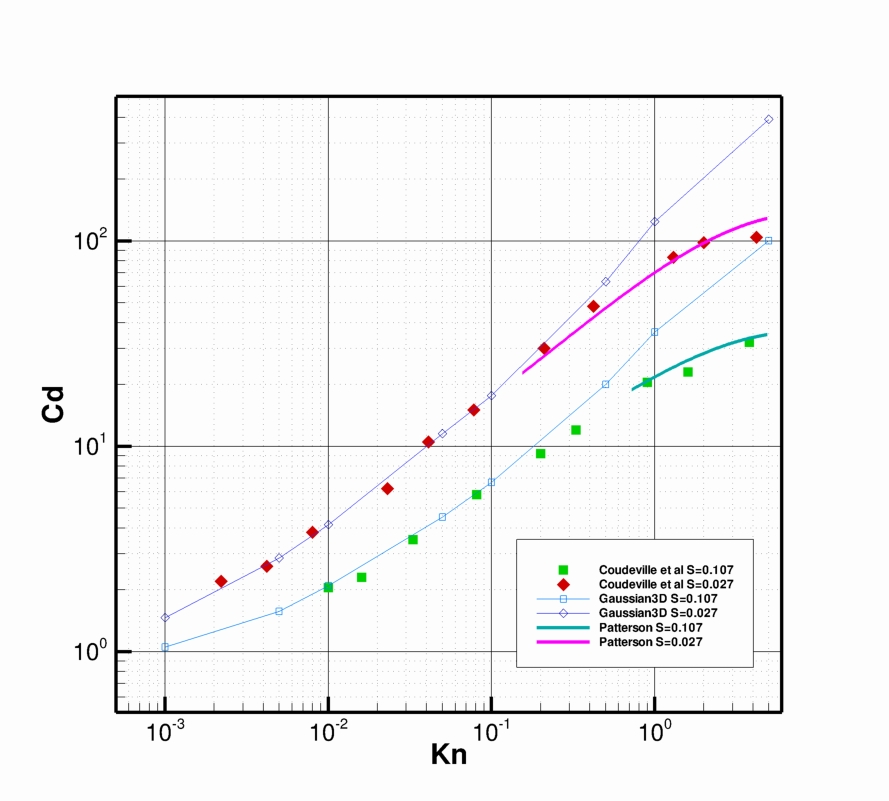
\includegraphics[width=0.45\textheight]{./figs/cylinder1.jpg}
    \caption{Drag coefficient for varying Knudsen numbers at two speed ratios: 
      Gaussian closure vs. experimental results.}
    \label{fig:cyl_d}
  \end{center}    
\end{figure}
%
\begin{figure}[t]
  \begin{center}
    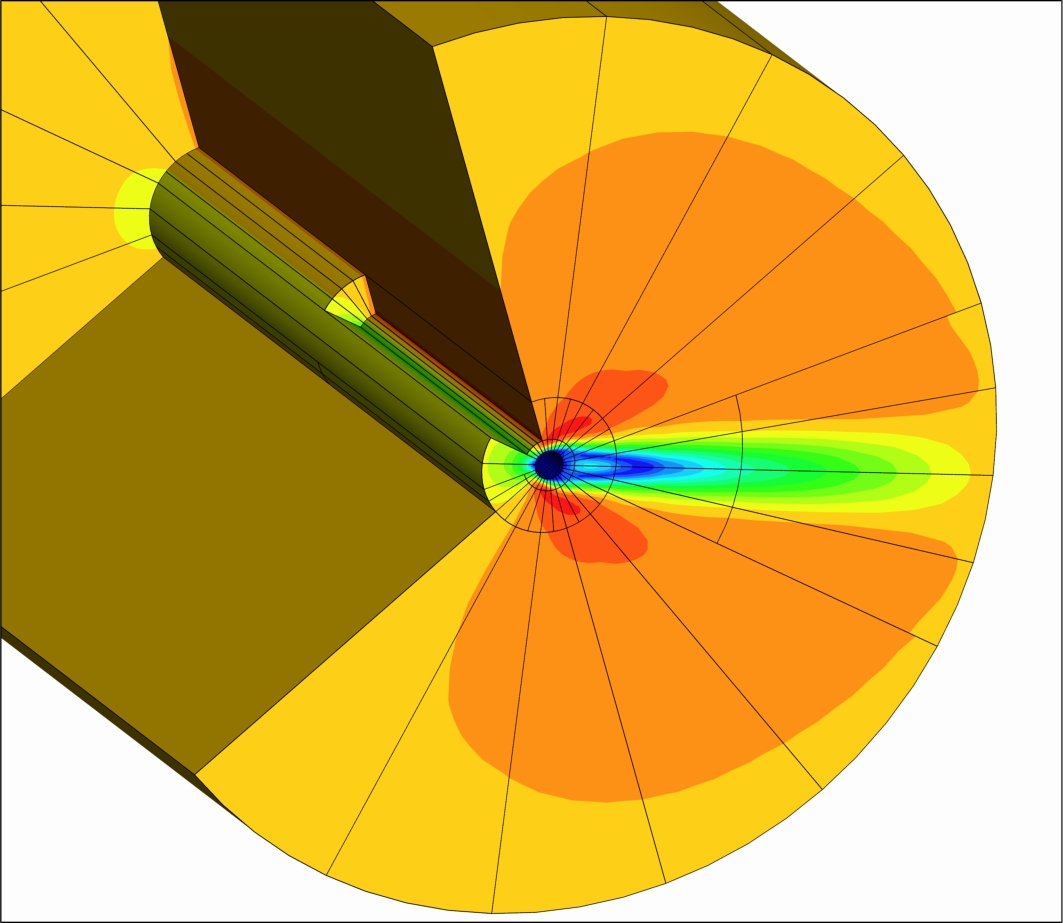
\includegraphics[width=0.3\textheight]{./figs/AMR_mesh2.jpg}
    \caption{A cutaway view of the two hundred eighty-eight radial mesh blocks created by the 
      AMR algorithm for immersed cylinder flow in the continuum regime with Mach number contours, 
      showing refined block structure at the surface of the cylinder and in the downstream regions}
    \label{fig:cyl_AMR}
  \end{center}    
\end{figure}
%
\begin{figure}[t]
  \begin{center}
    \subfigure[]{\label{subfig:cont-ex}
      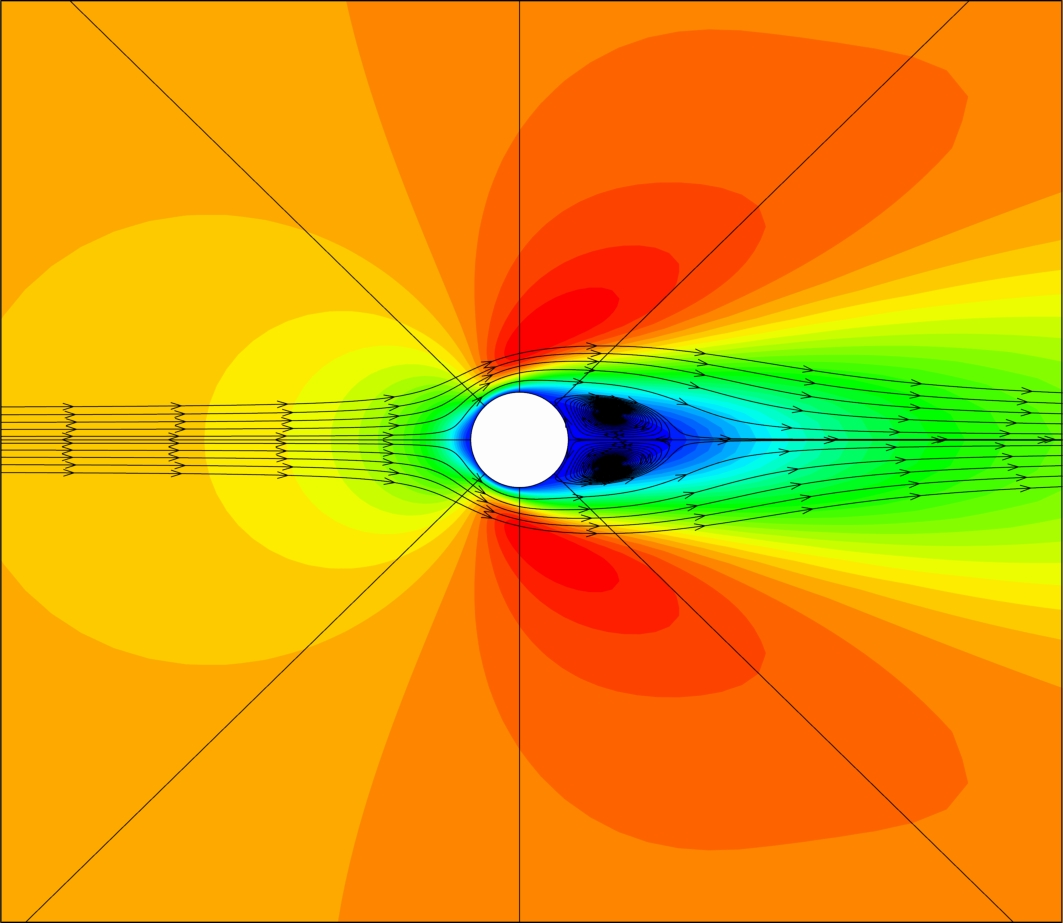
\includegraphics[width=0.22\textheight]{./figs/contexample.jpg}}
    \subfigure[]{\label{subfig:trans-ex}
      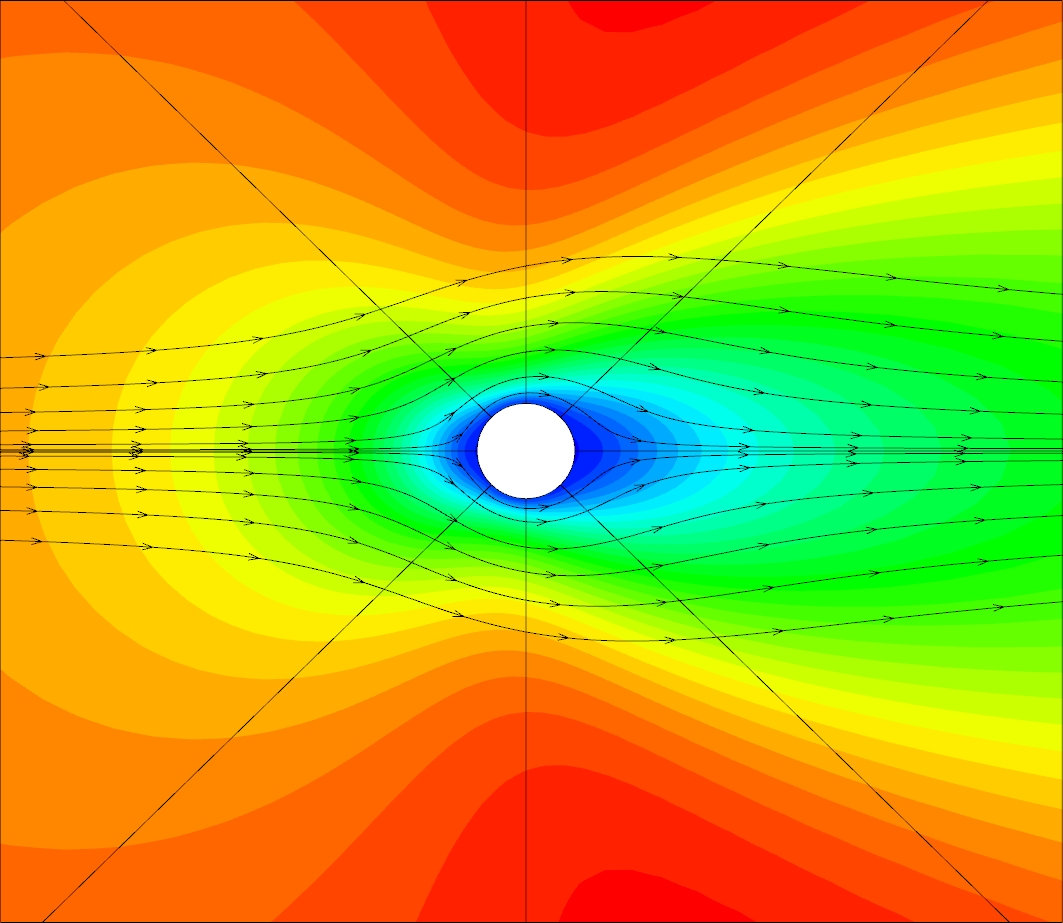
\includegraphics[width=0.22\textheight]{./figs/transexample.jpg}}
    %\\
    \subfigure[]{\label{subfig:free-ex}
      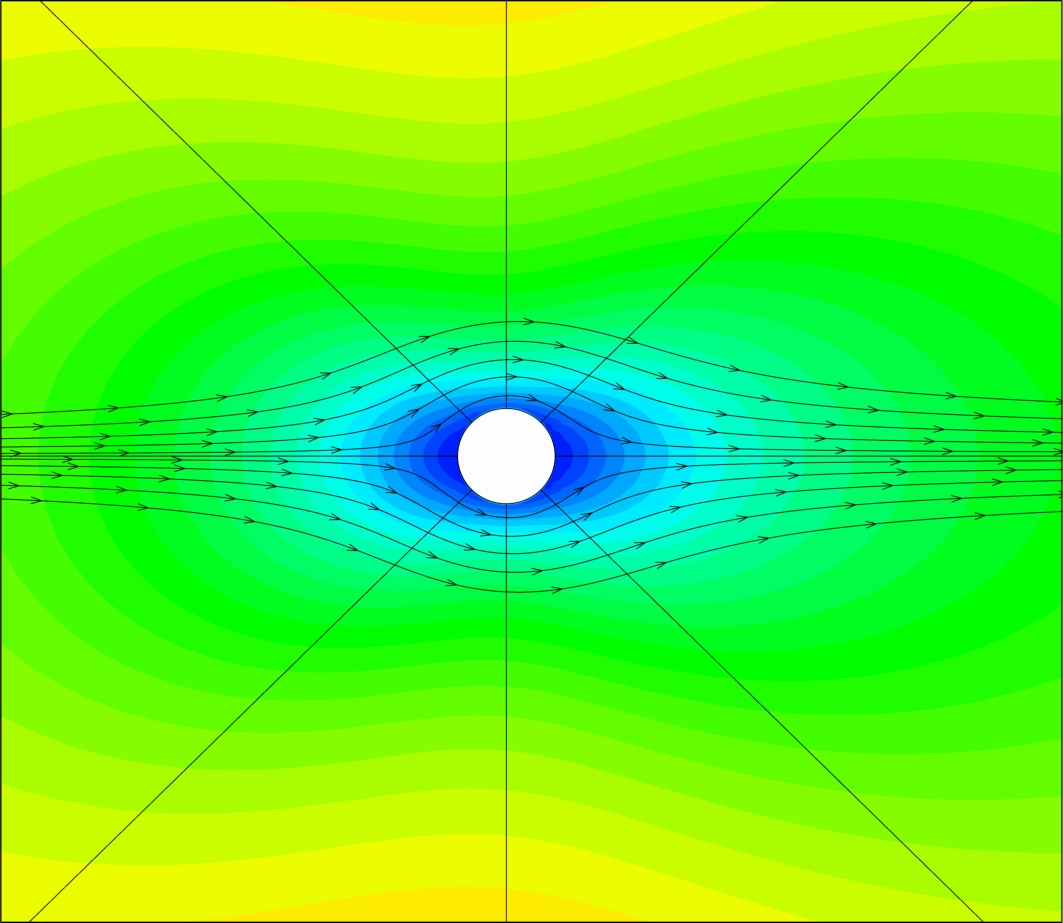
\includegraphics[width=0.22\textheight]{./figs/freeexample.jpg}}
    \caption{Comparison of x-directional velocity profile for immersed cylinder flow for various Knudsen numbers
      (a) $Kn = 1 \times 10^{-3}$,  
      (b) $Kn = 1 \times 10^{-1}$,
      (c) $Kn = 1. $
    }
    \label{fig:cyl_x}
  \end{center}    
\end{figure}
%
%%%%%%%%%%%%%%%%%%%%%%%%%%%%%%%%%%%%%%%%%%%%%%%%%%%%%%%%%%%%%%%%%%%%%%%%%%%%%%%%%%%%%%%%%%%%
%-------------------------------------------------------------------------------------------
% Flat Plate Boundary Layer Flow
%-------------------------------------------------------------------------------------------
%%%%%%%%%%%%%%%%%%%%%%%%%%%%%%%%%%%%%%%%%%%%%%%%%%%%%%%%%%%%%%%%%%%%%%%%%%%%%%%%%%%%%%%%%%%%
\subsection{Flat Plate Boundary Layer Development}\label{sec:flatplate} 
The Gaussian closure's ability to model slip flows and its effect on the boundary layer is 
shown here through the modeling of boundary layer development over a flat plate. Figure 
\ref{fig:flatplate_BL} compares the boundary layer profiles between the Knudsen 
number-independent Blasius solution~\cite{granger:1995} and solutions from the continuous 
$(Kn=2.6\times 10^{-5})$ and transition regimes $(Kn=2.6\times 10^{-1})$. Blasius proposed a 
relation between a non-dimensionalized velocity $u/U$ normalized to the free stream 
velocity, $U$, and a non-dimensional number $y \sqrt{\frac{U}{\nu x}}$ relating to the 
development of the boundary layer at a certain position above the plate. These 
non-dimensionalized numbers are calculated for both the continuous and transitional case 
for comparison purposes.

The continuum result from the Gaussian closure matches closely with the Blasius 
approximation with a zero slip velocity at the wall, while a transitional regime solution 
clearly shows a non-zero velocity at the wall. The ability to model slip flow effects 
without changing the boundary conditions of the problem is a powerful tool that the 
Gaussian closure can provide.
%
%% \begin{figure}[t]
%% \begin{center}
%% \includegraphics[width=0.5\textheight]{.figs/fig_flatplate.jpg}
%% \caption{Boundary layer development along a flat plate, with boundary layer thickness $\delta (x)$, 
%% velocity profile $u(x,y)$ inside the boundary layer, and the free stream velocity $U$.}
%% \label{fig:flatplate}
%% \end{center} 
%% \end{figure}
%
\begin{figure}[t]
  \begin{center}
    \subfigure[]{\label{subfig:continuum-flatplate}
      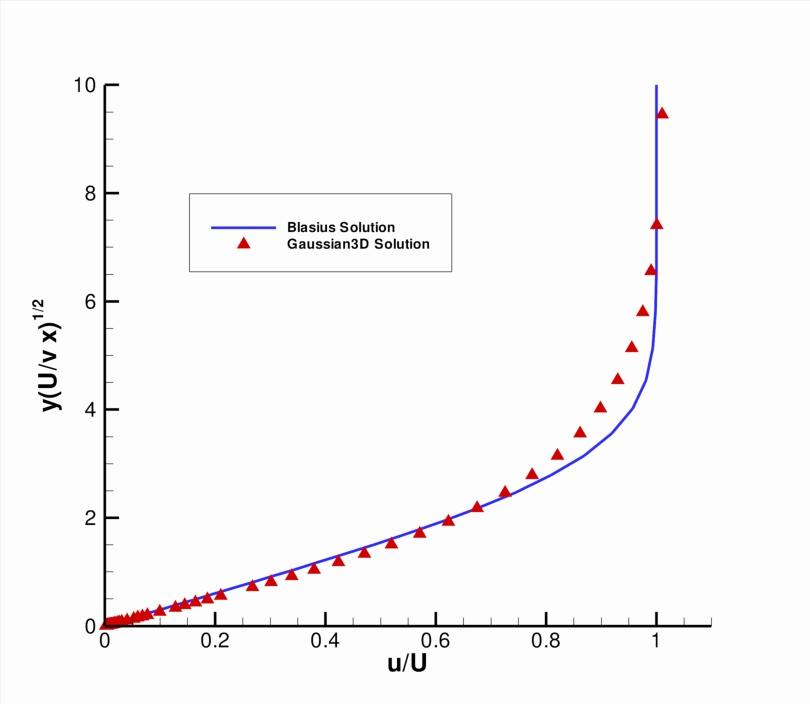
\includegraphics[width=0.35\textheight]{./figs/Kn000002.jpg}}
    \subfigure[]{\label{subfig:transition-flatplate}
      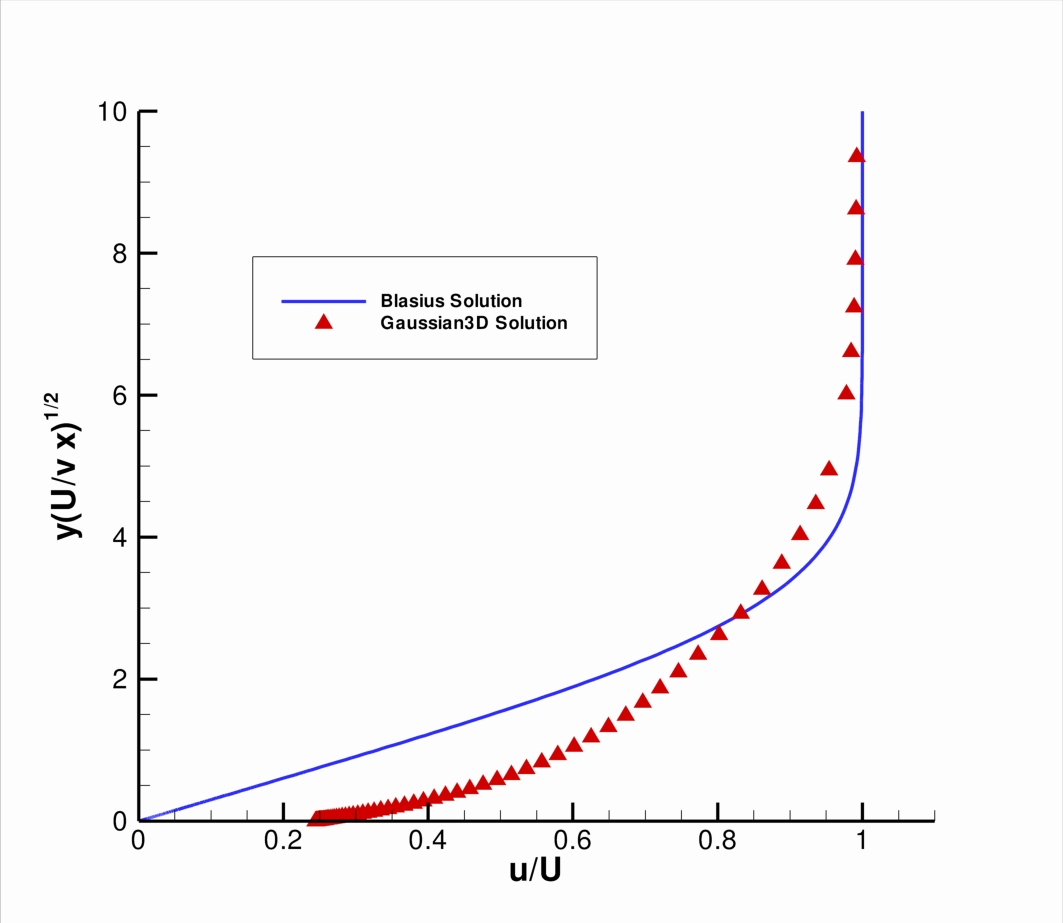
\includegraphics[width=0.35\textheight]{./figs/Kn02.jpg}}
    \caption{ 
      Flat plate normalized velocity distribution in developing boundary layer at varying Knudsen numbers
      (a) Continuum Regime, $Kn=2.6\times 10^{-5}$,  
      (b) Transition Regime, $Kn=2.6\times 10^{-3}$.
    }
    \label{fig:flatplate_BL}
  \end{center}    
\end{figure}
%

%%%%%%%%%%%%%%%%%%%%%%%%%%%%%%%%%%%%%%%%%%%%%%%%%%%%%%%%%%%%%%%%%%%%%%%%%%%%%%%%%%%%%%%%%%%%
%-------------------------------------------------------------------------------------------
% Planar Couette Flow
%-------------------------------------------------------------------------------------------
%%%%%%%%%%%%%%%%%%%%%%%%%%%%%%%%%%%%%%%%%%%%%%%%%%%%%%%%%%%%%%%%%%%%%%%%%%%%%%%%%%%%%%%%%%%%
\subsection{Planar Couette Flow}\label{sec:couette}
Planar Couette flow is studied here to illustrate the Gaussian closure's ability to model 
boundary layer and shear stress evolution in various flow regimes. For this particular 
problem, the two plates are moving at 30 m/s in opposite directions in argon at 288k in 
standard pressure, and the setup is extruded in the $z$ direction. Figure 
\ref{subfig:couette-slipv} shows the non-dimensionalized velocity $\frac{u}{U}$, where $u$ 
is the fluid velocity at the wall and $U$ is the wall velocity, versus the Knudsen number 
based on the separation of the two plates. The continuum solution using the Navier-Stokes 
equations with no extra treatment for slip flows calculates the fluid velocity at the wall 
to be equal to the velocity of the wall regardless of Knudsen number. The free molecular 
solution generates an infinite slip velocity at the wall, with the fluid velocity at the 
wall equal to zero for all flows. Lees solution (1959)~\cite{vincenti:1975} provides an 
analytical solution to this problem that predicts the slip velocity and shear stress at 
the wall, gradually transitioning from the continuum result to the free-molecular. The 
Gaussian solution is capable of modeling the formation of a slip velocity and follows Lees 
solution closely for a wide range of Knudsen numbers.
%
%% \begin{figure}[t]
%% \begin{center}
%% \includegraphics[width=0.5\textheight]{./figs/fig_couette_diagram.jpg}
%% \caption{Two-dimensional setup of the Couette flow problem. For the three-dimensional modeling, 
%% this setup is extruded out through this plane.}
%% \label{fig:couette}
%% \end{center}    
%% \end{figure}
%
The shear pressure profile for the same problem can be seen in Figure 
\ref{subfig:couette-shear}. For comparison purposes, the shear stresses are normalized to 
the free molecular solution as $\frac{\tau_{xy}}{\rho U \sqrt{\frac{2kT}{\pi m}}}$. Use of 
the continuum formulation predicts an ever-increasing shear stress with increasing Knudsen 
number, while the free-molecular shear stress remains constant regardless of Knudsen 
number. The Gaussian solution predicts a smooth transition between the continuum and 
free-molecular solutions and is in close agreement with the analytical solution by Lees. 
%
\begin{figure}[t]
\begin{center}
\subfigure[]{\label{subfig:couette-slipv}
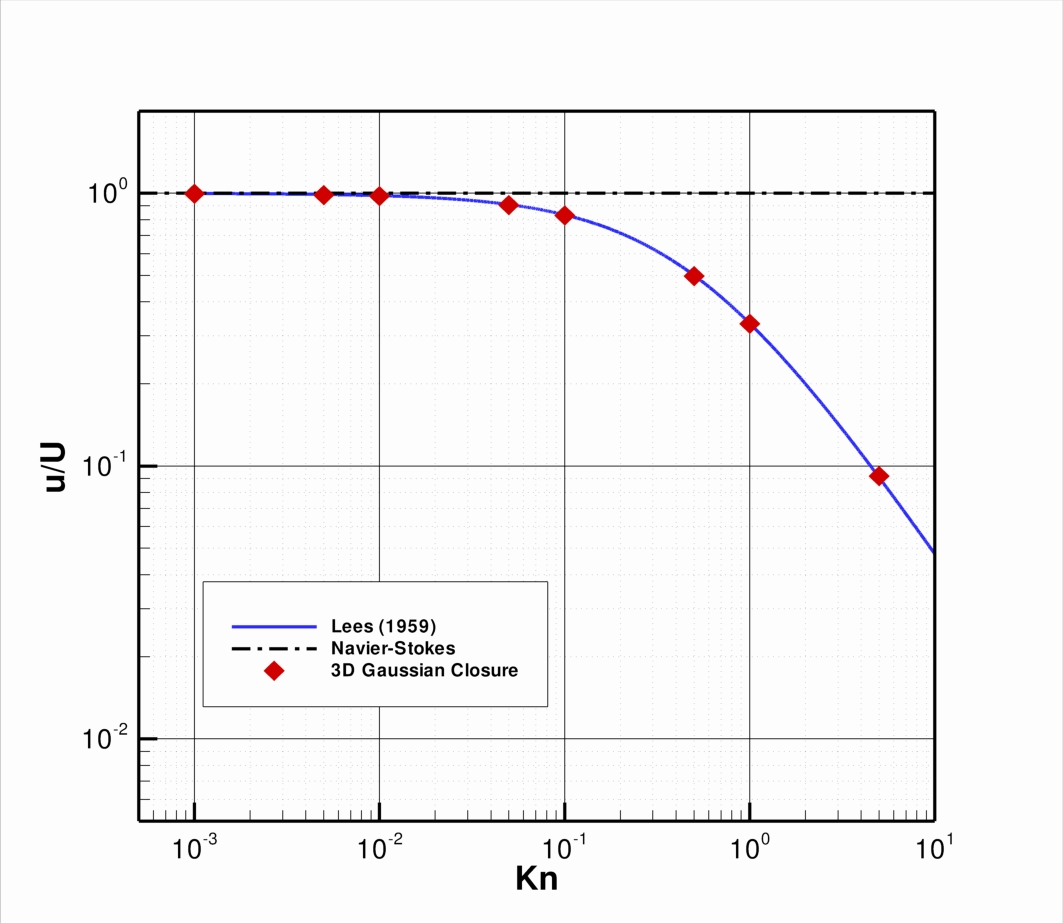
\includegraphics[width=0.35\textheight]{./figs/slip_velocity.jpg}}
\subfigure[]{\label{subfig:couette-shear}
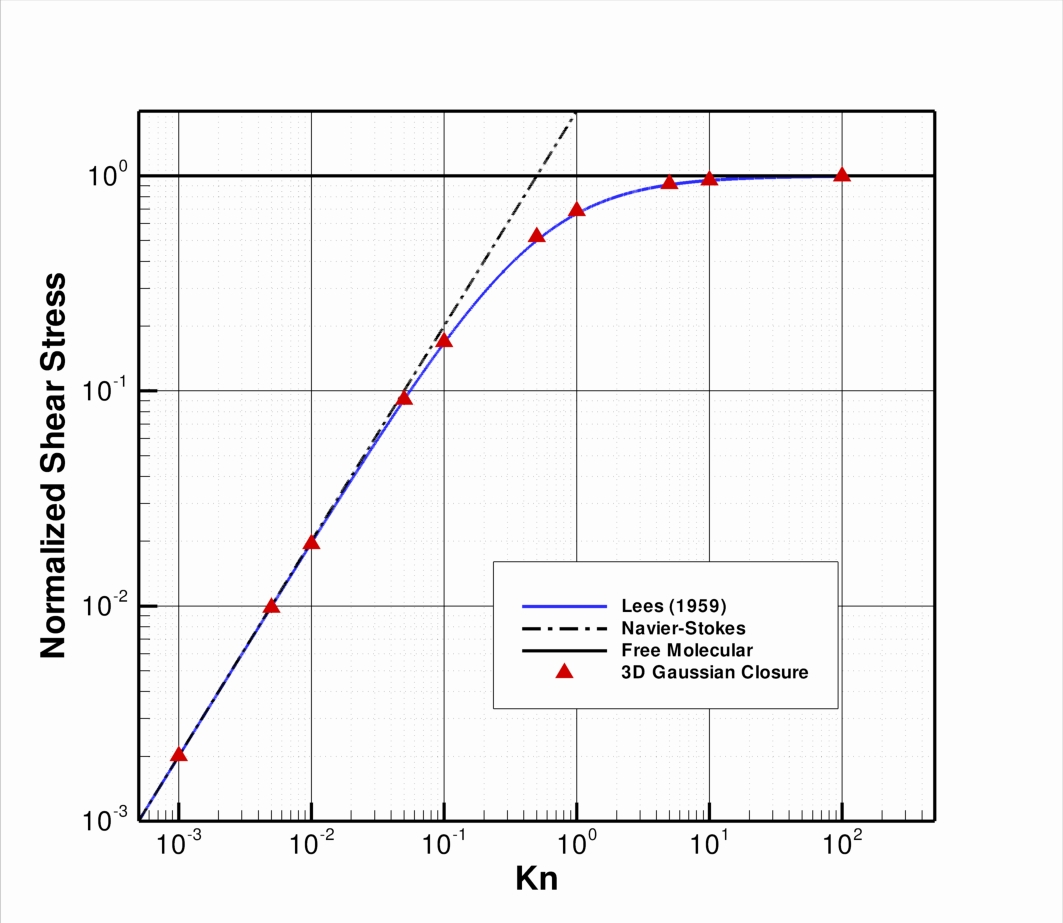
\includegraphics[width=0.35\textheight]{./figs/shear_stress.jpg}}
\caption{ 
(a) Normalized fluid velocity at the wall vs. Knudsen number. Note that the free-molecular 
solution gives $u=0$ at the wall regardless of Knudsen number,  
(b) Normalized shear stress at the wall vs. Knudsen number.
}
\label{fig:couette-data}
\end{center}    
\end{figure}
%

% ---------------------------------------
% SUMMARY PROGRESS TO DATE AND FUTURE WORK
% ---------------------------------------
\section{Summary of Progress to Date and Future Work}

\subsection{Progress to Date}

\begin{tabular}{|l|c|} \hline
\multicolumn{1}{|c|}{\bf{Task}} & \multicolumn{1}{|c|}{\bf{Completion Date}} \\

\hline Completion of 3D Gaussian moment closure code & October 2010 \\

\hline Completion of models for 3D Gaussian closure: & December 2010 \\ 
immersed cylinder, flat plate boundary layer, couette &\\

\hline Learning Newton-Krylov-Schwarz mathematical foundations & January 2011 \\

\hline Preliminary testing for immersed cylinder applied on NKS, no heat transfer & January 2011 \\

\hline Derivation of heat transfer terms for Gaussian closure & March 2011 \\

\hline
\end{tabular}

\subsection{Future Work}

\begin{tabular}{|l|c|} \hline
\multicolumn{1}{|c|}{\bf{Task}} & \multicolumn{1}{|c|}{\bf{Completion Date}} \\

\hline Learning heat transfer incorporation into Gaussian closure and & April 2011 \\ 
computational effects on solution &\\

\hline Convective Heat Transfer (MIE1212); heat transfer for internal and 
& April 2011 \\ external flows, developing boundary conditions, final paper &\\

\hline Introduction to Modern Flow Control (AER1308); turbulence models, &
April 2011 \\ flow control techniques, final paper &\\

\hline 2D Gaussian moment closure code: example analysis for &
May 2011 \\ heat transfer effects, application towards 3D code &\\

\hline AIAA Conference paper/presentation: NKS solver applied to Gaussian  & June 2011 \\ 
closure without heat transfer effects &\\

\hline Adapting 3D Gaussian moment closure code for other mesh geometries & August 2011 \\

\hline Incorporation of heat transfer terms in 3D Gaussian moment closure code, &
January 2012 \\ testing and validation, comparison with experimental results &\\

\hline Investigation of alternate regularization methods and their effect on &
June 2012 \\ computational time and accuracy &\\

\hline Thesis write-up &
March 2014 \\ \hline

\end{tabular}

%\newpage
\bibliographystyle{aiaa} \bibliography{journals-full,cfd,myrefs}
\end{document}
